\documentclass[11pt]{amsart}
%%% WARNING: Do NOT change the page size, fonts, or margins!  Penalties will apply.


\usepackage{graphicx}
\usepackage{amssymb, amsmath, amsthm}
\usepackage{places}
\usepackage{wrapfig,floatrow}
\usepackage{varwidth, caption, subcaption} %enables \FloatBarrier, which prevents figures and tables from going below it.
%\usepackage{hyperref} %makes cross references into hyperlinks. 
\usepackage{amsmath, amssymb, amsthm, amsfonts, algpseudocode, algorithm, bbm, color, fixmath, float, graphicx, hyperref, listings, mathrsfs, mathtools, subfig, times}

%Needed commands
\newcommand*{\w}{\mathbf{w}}
\newcommand*{\x}{\mathbf{x}}
\newcommand*{\y}{\mathbf{y}}
\newcommand*{\z}{\mathbf{z}}
\newcommand*{\R}{\mathbb{R}}
\newcommand*{\E}{\mathbb{E}}
\newcommand*{\0}{\mathbf{0}}
\newcommand*{\minimizer}{\mathbf{x}^*}
\newcommand*{\dprime}{{\prime\prime}}
\newcommand{\li}[1]{\lstinline[prebreak=]!#1!}
\newcommand{\pseudoli}[1]{\lstinline[style=pseudo]!#1!}
\newcommand{\trp}{^{\mathsf T}} 
\newcommand{\im}{{i\mkern1mu}}
\newcommand{\Real}{\mathchardef\Re="023C}
\newcommand{\Imag}{\mathchardef\Im="023D}
\newcommand\norm[1]{\left\lVert#1\right\rVert}
\newcommand*\diff{\mathop{}\!\mathrm{d}}
\newcommand*\Eval[3]{\left.#1\right\rvert_{#2}^{#3}}

%Operators
\DeclareMathOperator{\argmin}{argmin}
\DeclareMathOperator{\argmax}{argmax}

%Link set up
\hypersetup{
    colorlinks=true, %set true if you want colored links
    linktoc=all,     %set to all if you want both sections and subsections linked
    linkcolor=blue,  %choose some color if you want links to stand out
    pdftitle={RL Notes},
    pdfpagemode=FullScreen
}

\endinput

%%% WARNING: Do NOT change the page size, fonts, or margins!  Penalties will apply.
%%% WARNING: Do NOT change the page size, fonts, or margins!  Penalties will apply.
% The Effect of Chemotherapy and Immunological Response on Breast Cancer Growth
\title{Insert Some Cool Title Here}
\author{R. Gee, H. Fetzer, N. Suyama, J. Humpherys, O.J. Escobar}
\date{October 29 2024} % or use \today

\begin{document}
\maketitle % this actually makes the title

\begin{abstract}
Place abstract here. The abstract summarizes in one paragraph the main question and conclusions draw from your investigation.
\end{abstract}

%% First Section
\section{Background/Motivation}

Mathematical oncology employs math to study cancer.
``It [serves] as a bridge between $\ldots$ the biologist, and the practicing clinician" (Dr. Rockne and MD Scott) \cite{IntroMathOnc}.
Tumor growth modeling is an application of mathematical oncology, which seeks to understand and model the properties that govern cancer growth, and the relationship between cancer, treatment and the immune system.

The purpose of tumor growth modeling is to: (1) develop an uninhibited tumor growth model, (2) model the results of external factors like immune response or treatment, and (3) model tumor and other immune resistance to treatments.
Models measure \textit{tumor burden}, denoted $T$, (see\ \ref{appendix: defs} for definitions), as a function of time $t$.
Commonly used models include linear, exponential, and logistic models (see\ \ref{appendix: models} for equations).
However, these are not accurate to the growth of most observed cancers \ \cite{Steb23}, which involve a slow exponential rate of increase and a slow convergence to a maximal tumor burden.
The purpose of these general growth models is to develop more personal cancer treatment to individuals.\ \cite{YinMoes}

Most cancers are treated through a combination of surgery, chemotherapy, and radiation therapy.
Surgery removes as much as the cancer as possible, but is unsuited for modeling because it creates discontinuities.
Therefore, although surgery is the primary treatment for breast cancer, we will focus on modeling chemotherapy (see\ \ref{appendix: defs}) since it is the most common treatment supplement to surgery.

Most models for tumor growth in response to chemotherapy show the effect of a single dose of chemotherapy on cells at specific cell-cycles and seek to model the resistance of a tumor to the given drug.
A full chemotherapy treatment cycle includes a sum of multiple doses that decay over time, and may include sudden changes in the tumor growth as modeled by Nave\ \eqref{eq: NavePersonalChemo}.
Ophir Nave described an interaction between the chemotherapy drug and both the immune system and cancer itself \ \cite{NAVE2022e09288}.
An exponential decay of the drug best models the rapid effect that chemotherapy has on the tumor burden (e.g.\ \eqref{eq:PanettaExpDec}).
Unfortunately, these models often ignore the effect of cancer treatment on other parts of the body, which we expect to have a similar response to cancer cells.
Thus, we attempt to find an expression for chemotherapy that affects both tumors and the immune system.

The immune system is the body's natural defense against foreign bacterias or other abnormal cells (including cancer cells), which includes many different cell types, of which we will focus on two.
Most models, as in\ \ref{eq: dePillisTumorImmuno} or\ \ref{eq: AlharbiTumorImmuno}, look at the response of the entire immune system to cancer, rather than the contributions of each cell type.
While working generally, it suffices to show the interaction as a whole, but as mentioned by de Pillis et. al, ``in some applications, it is not sufficient to represent the immune response with a single homogeneous population of effector killer cells\ \cite{dePillis2014461}."
Thus, a good model for a certain type of cancer, should show interactions between the cells affecting that cancer.

The immune system has many types of cells, but NK cells and CD8$^+$ cells alone kill breast cancer cells\ \cite{Amens21}.
Hence modeling for tumor-immunological responses focuses on behavior of \textit{natural killer} cells (NK), which make up an innate immune system, and \textit{cytotoxic T}-cells (CD8$^+$), which form an adaptive immune system (see\ \ref{appendix: defs}).
CD8$^+$ cells are trained to kill cancer by the NK cells, which forms a relation between NK, CD8$^+$, and cancer cells.

Immune system and tumor interactions can be modeled by \textit{Michaelis-Menten kinetics} (see\ \ref{appendix: defs}), which models interactions, like immune system response to cancer cells, tumor cells affecting the immune system, or infection of normal cells by tumor cells\  \cite{math8081285}.
Any model looking into the interaction of a tumor with the immune system should consider similar interactions to these.


Given the difficulty of modeling tumor growth in general, the intricacies of chemotherapy, and the complexity of immune-tumor interactions, we can understand why creating a completely general model of any cancer is arduous.
Thus, we narrow our focus and attempt a simpler model that follows the previous guidelines.
Since the National Cancer Institute records it as having the most number of cases as of 2024, we decided to focus on breast cancer.
Our tumor growth modeling consists of a Gompertz growth model with a specific neoadjuvent chemotherapy treatment, and an immune response given by NK and CD8$^+$ cells.


%% Second Section 
\section{Modeling}

%% Third Section
\section{Results}

%%Fourth Section
\section{Analysis/Conclusions}


\newpage
\appendix

%%%%%%%%%%%%%%%%%%%%% Appendix A: Graphs %%%%%%%%%%%%%%%%%%%%%
\section{Supplemental Graphs}
\label{appendix:graphs}
In this section, we give more graphs that help our analysis as supplementary information to the main points and graphs given in the paper.
\begin{figure}[H]
\vspace{-2mm}
\begin{center} %Put your images in a figure like this
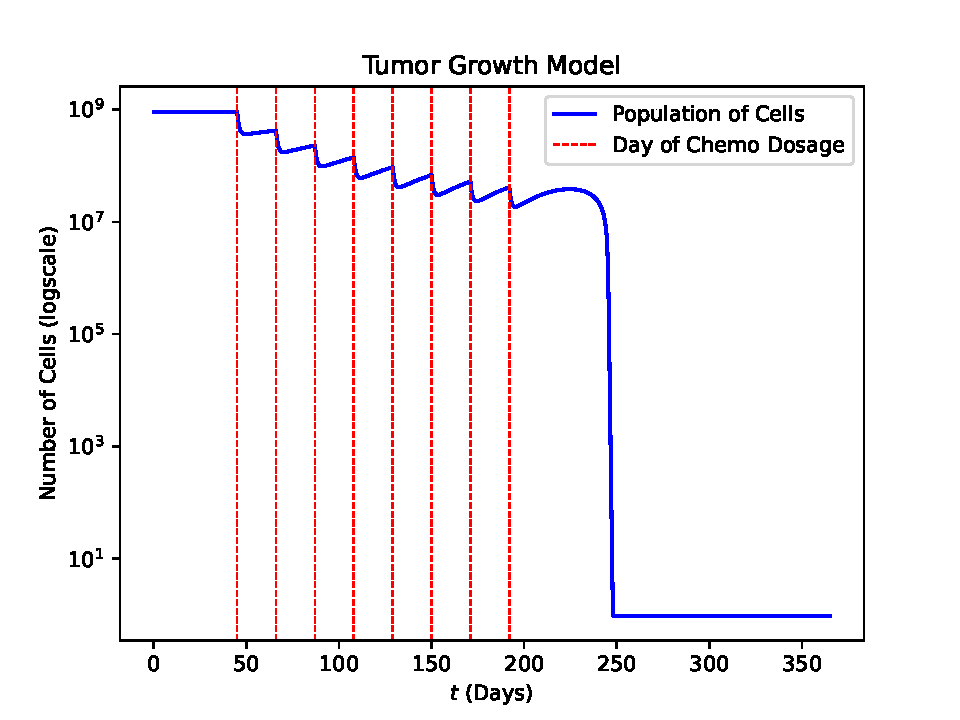
\includegraphics[scale=0.6]{./images/growth_8T_3W_C45_semiy.pdf} % Better to make them pdfs than png or gif or jpeg
\end{center}
\caption{The growth of breast cancer, in a semilog scale for $T$, as modeled by \eqref{eq:unifiedmodel}. Compare to Figure~\ref{fig:FullODE}. This graph helps us appreciate the actual death of cancer to near zero.}\label{fig:FullODE_semiy} % for automatic cross referencing
\end{figure}

\begin{figure}[H]
\begin{center} %Put your images in a figure like this
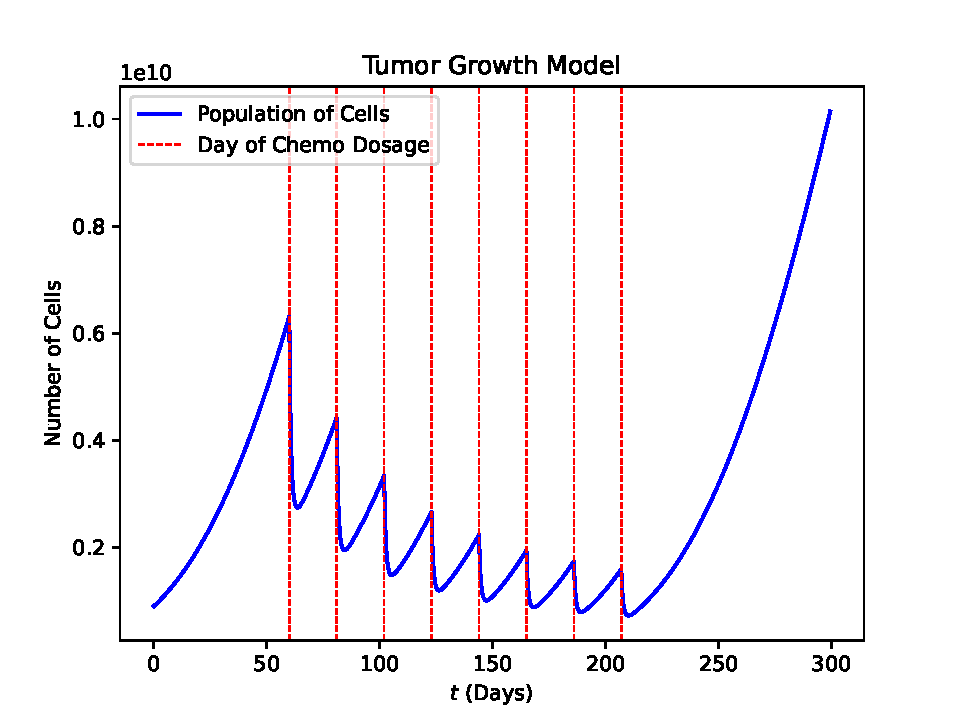
\includegraphics[scale=0.6]{./images/abnormal_growth_8T_3W.pdf} % Better to make them pdfs than png or gif or jpeg
\end{center}
\caption{Abnormal growth given by an abnormally big tumor capacity of size at least $91$mm in diameter.}\label{fig:abnormal_growth} % for automatic cross referencing
\end{figure}

\begin{figure}[H]
\begin{center} %Put your images in a figure like this
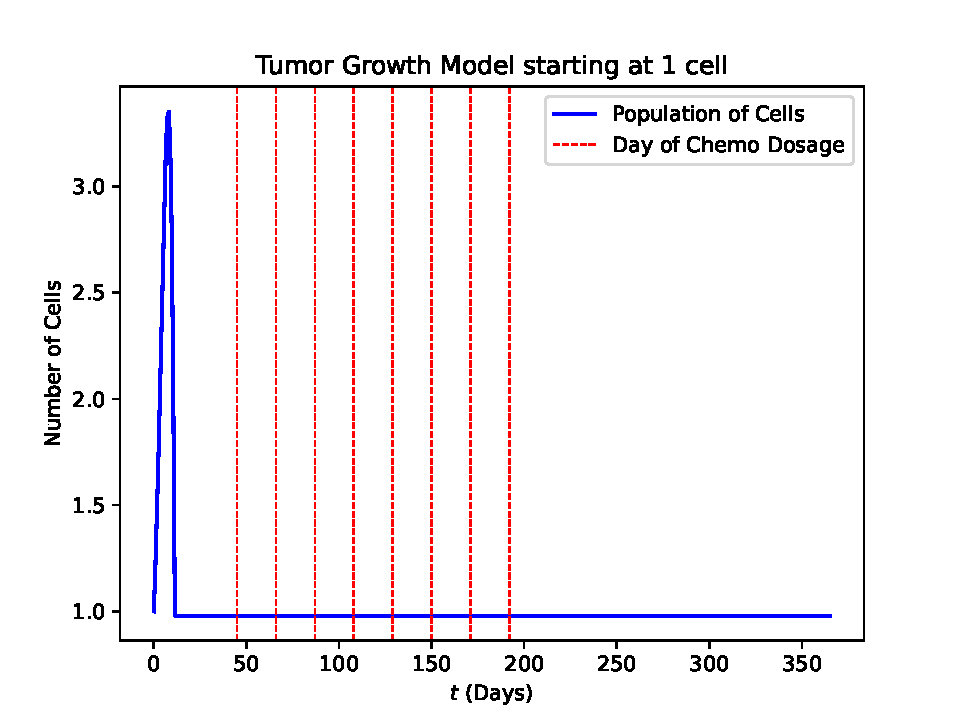
\includegraphics[scale=0.6]{./images/growth_1cell.pdf} % Better to make them pdfs than png or gif or jpeg
\end{center}
\caption{Tumor growth starting from 1 cell.}\label{fig:1cellgrowth} % for automatic cross referencing
\end{figure}

Here we plot the differential equations of the immune system. 
We get our initial values from a plot in the paper where we got the differential equations. 
In the paper published, the populations only go to about 35 days. 
Below we've created similar plots, but as we increase the time beyond 35 days, 
we start to see some problems, which we will address in the analysis/conclusions section.

\begin{figure}[H]
\begin{center} %Put your images in a figure like this
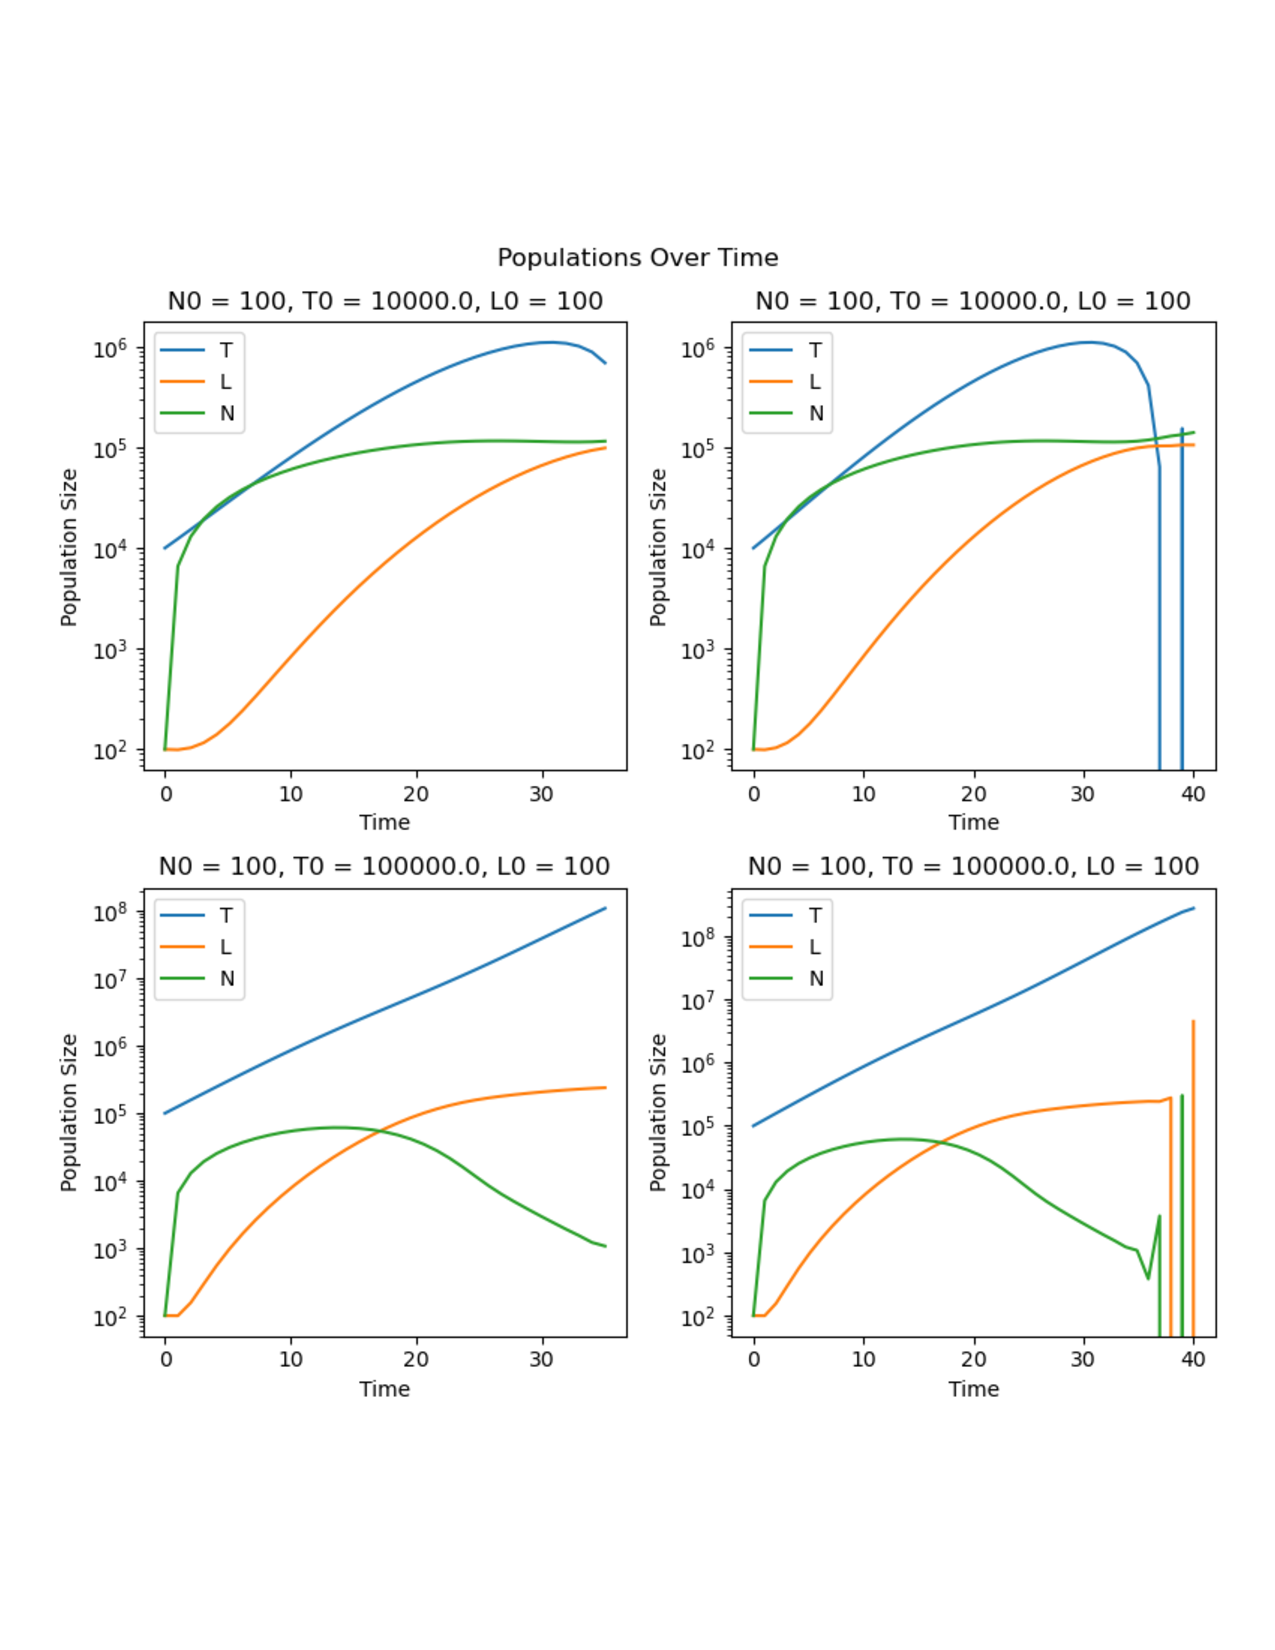
\includegraphics[scale=.6]{./images/forward_immune.pdf} % Better to make them pdfs than png or gif or jpeg
\end{center}
\caption{Various plots of the populations for different initial values}
\label{fig:forward} % for automatic cross referencing
\end{figure}


%%%%%%%%%%%%%%%%%%%%% Appendix B: Definitions %%%%%%%%%%%%%%%%%%%%%
\section{Definitions}
\label{appendix: defs}
The following definitions are derived from the National Cancer Institute, unless otherwise stated
\begin{itemize}
	\item Adaptive Immune System: the part of the immune system that specifically targets the germs or foreign substances that are causing an infection. In order to do this, this system needs to first recognize the substance as such. Therefore, this system is slower and needs training. CB8$^+$ cells are part of this system.
	\item Cancer:  a term for diseases in which abnormal cells divide without control and can invade nearby tissues
	\item Chemotherapy: a cancer treatment where drugs are used to kill cancer cells or stop them from dividing
		\begin{itemize}
			\item Neoadjuvent Chemotherapy: chemotherapy administered before the primary treatment of the tumor is performed. Typically, surgery is the primary treatment. Its main goal is to shrink the tumor so that it is easier to remove.
			\item Adjuvent Chemotherapy: Chemotherapy administered after primary tumor treatment is administered. Its intent is to lower the risk of the cancer returning.
		\end{itemize}
	\item Cytotoxic/CD8$^+$ T-cell: is a T-lymphocyte that kills or infected cells or cells that are damaged in other ways. They are not natural killers and as such have to be trained to kill cancer. (Mayo clinic)
	\item Innate Immune System: the part of the immune system that is the first line of defense against intruders or unknown foreign cells in the body. It responds to all foreign substances in the same manner (National Library of Medicine). It can be thought of as "kill first, ask questions later." NK cells are part of this system.
	\item Log-kill Hypothesis: when growth of a cancer is exponential—increasing by a constant fraction of itself every fıxed unit of time—then in the presence of effecive anticancer drugs it also shrinks by a constant fraction \cite{LogKill}
of itself
	\item Remission: A decrease in or disappearance of signs and symptoms of cancer. In partial remission, some, but not all, signs and symptoms of cancer have disappeared. In complete remission, all signs and symptoms of cancer have disappeared, although cancer still may be in the body.
	\item Treatment cycle: the regular and repeated interval of time between each new dose of a chemotherapy drug. A cycle comprises of a rest period to allow the body to heal from the effects until the new dose is given. This information was retrieved from the American Cancer Society and\ \cite{CALEY2012186}.
	\item Tumor: an abnormal mass of tissue that forms when cells grow and divide more than they should or do not die when they should. Tumors may be \textit{benign} (not cancer) or \textit{malignant} (cancer). For this project, defined the tumor burden as the number of cancer cells in the body.
	\item Tumor burden: the size of a tumor or number cancer cells. This is the total amount of cancer found in the body.
        \item Natural Killer Cell (NK Cell): A type of immune cell that has granules (small particles) with enzymes that can kill tumor cells or cells infected with a virus. A natural killer cell is a type of white blood cel
\end{itemize}


%%%%%%%%%%%%%%%%%%%%% Appendix C: Other Models %%%%%%%%%%%%%%%%%%%%%
\section{Models}
In this section, we describe and give equations we have referenced throughout our work.

\label{appendix: models}
\begin{itemize}

	\item Tumor Growth Models:
		\begin{itemize}
	\item Linear growth: 
		\begin{equation}
			\frac{\diff T}{\diff t} = k,
			\label{eq: lin}
		\end{equation}
		where $k$ is the growth rate
	\item Exponential Growth:
		\begin{equation}
			\frac{\diff T}{\diff t} = kT \label{eq: exp}
		\end{equation}
	 or with a death rate constant of $d$, $\frac{\diff T}{\diff t} = (k-d)T$
	\item Logistic Growth: 
		\begin{equation}
			\frac{\diff T}{\diff t} = kT \biggl(1- \frac{T}{T_{\max}}\biggr)\label{eq: logistic},
		\end{equation}
		where $T_{\max}$ is the max size a tumor can be, which is equivalent to the carrying capacity.
		\end{itemize}
		
	\item Chemotherapy Models: 
		\begin{itemize}
			\item Exponential Decay: Pillis and Radunskaya modeled the mix of immunotherapy and chemotherapy on tumor growth. In particular, they modeled the drug as an exponential decay given by 
				\begin{equation}
					G_M = -\gamma M \label{eq: Pillis},
				\end{equation}
				where $M=M(t)$ is the concentration of the drug in the bloodstream at some time $t$.
				
			\item Panetta also used an exponential but considering the frequency between doses as
				\begin{equation}
					g(t) = h e^{-\gamma(t-n-\tau)} \label{eq:PanettaExpDec},
				\end{equation}
				where $g(t)$ is the effects of the chemotherapy drug, $\gamma$ is the decay of the drug, $n$ is number of doses, and $\tau$ is the period between doses.
				
			\item Personalized treatment: Ophir Nave modeled a personalizable treatment plan as 
				\begin{equation}
					\mathscr{F} = \sum_{k=0}^n q(t-mk) \mathscr{H} (t-mk)e^{\frac{t-mk}{0.5}}\label{eq: NavePersonalChemo},
				\end{equation}
				where $n$ is the duration of the treatment, $m$ is the interval between treatments, and $\mathscr{H}$ a unit step function.
		\end{itemize}
	\item Immunological Response Models:
		\begin{itemize}
			\item Pillis, Radunskaya, Wiseman:\\
                    			$\frac{dT}{dt} = aT(1-bT) - cNT - D\\$
                    			$\frac{dN}{dt} = \sigma - fN +\frac{gT^2}{h + T^2}N - pNT\\$
                    			$\frac{dL}{dt} = - mL +\frac{jD^2}{k + D^2}L - qLT + rNT\\$
                    			$D = d\frac{(L/T)^\lambda}{s + (L/T)^\lambda}T$\\
                    		Where we define each constant:
                   		 \begin{itemize}
                    			\item a = $5.14 \times 10^{-1}$ has units $\text{day}^{-1}$ is the tumor growth rate
                    			\item b = $1.02 \times 10^{-9}$ has units $\text{cell}^{-1}$ where  $\frac{1}{b}$ is the tumor carrying capacity.
                   		 	\item $N_{NR}$ = $3.23 \times 10^{-7}$ has units $\text{cell}^{-1}\text{day}^{-1}$ is the fractional cell kill(see appendix) rate of NK cells against tumors.  
                   		 	\item $sigma = 1.3 \times 10^4$ has units $\text{cells} \text{day}^{-1}$ is the constant NK cells production.
                   		 	\item $N_d = 4.12 \times 10^{-2}$ has units $\text{day}^{-1}$ is the natural death rate of NK cells.
                   		 	\item $g = 2.5 \times 10^-2$ has units $\text{day}^{-1}$ is the max NK recruitment
                   		 	\item $h = 2.02 \times 10^7$ has units $\text{cell}^2$ is the steepness coefficient of the NK recruitment curve.
                   		 	\item $p = 1.00 \times 10^{-7}$ has units $\text{cell}^{-1}\text{day}^{-1}$ is the rate at which tumors incapacitate NK cells
                   		 	\item $m = 2.00 \times 10^{-2}$ has units $\text{day}^{-1}$ is the natural death rate of CD8+ cells.
                   		 	\item $j = 3.75 \times 10^{-2}$ has units $\text{day}^{-1}$ is the max CD8+ recruitment rate, and the constant $k = 2 \times 10^7$ has units $\text{cell}^2$ is the steepness coefficient of the CD8+ recruitment curve.
                   		 	\item $L_R = 2 \times 10^7$ has units $\text{cell}^2$ is the steepness coefficient of the CD8+ recruitment curve.
                   		 	\item $q = 3.42 \times 10^{-10}$ has units $\text{cell}^{-1}\text{day}^{-1}$ is the rate that tumors deactivate CD8+ cells.
                   		 	\item $r =1.1 \times 10^{-7} $ has units $\text{cell}^{-1}\text{day}^{-1}$ is the rate at which those CD8+ cells are produced. 
                    			\item $d = 5.80$ has units $\text{day}^{-1}$ is the saturation level of fractional tumor cell kill by CD8+ T cells
                    			\item $s = 2.5 \times 10^{-1}$ has no units, and is the steepness of the curve which determines the Tumor vs. CD8+ cell competition. Lastly, \item $\lambda = 1.36$ has no units. 
				\end{itemize}
			\item Alharbi \& Sham Rambely: their modeling equations looked at the interaction of tumor cells and the immune system, $I$, as a whole as well as normal cells , $N$, (non-immune, non-tumor cells). They described the relationships by (using a logistic growth for tumor $T$):
				\begin{eqnarray}
					\begin{aligned}
						\frac{\diff N}{\diff t} &= rN(1-\beta_1 N) - \eta NI - \gamma NT \\
						\frac{\diff T}{\diff t} &= \alpha_1T(1-\alpha_2T) + \beta_2 NT - \alpha_3 T1 \\
						\frac{\diff I}{\diff t} &= \sigma - \delta I _ \frac{\rho N I}{m+N} + \frac{\rho_1 TI}{m_1 + T} - \mu NI - \mu_1 TI \label{eq: AlharbiTumorImmuno}
					\end{aligned}
				\end{eqnarray}
			\item dePillis et. al: they modeled the primary interaction between effector cells, $E$, like CB8$^+$, and the tumor, $T$ by using logistic growth and 
				\begin{eqnarray}
					\begin{aligned}
						\frac{\diff T}{\diff t} &= a_1T(1-b_1T) - c_2ET - c_3NT - k_2(1-e^{-u}) \\
						\frac{\diff N}{\diff t} &= a_2(1-b-2N) - c_4NT - k_3 (1-e^{-u})\label{eq: dePillisTumorImmuno}
					\end{aligned}
				\end{eqnarray}
		\end{itemize}
	\item Growth-Chemo-Immune PDE System: Ansarizadeh, Singh, and Richards modeled tumor cells using a system of PDEs. Specifically, they used a logistic model for the normal cells $N$, tumor $T$, immune $I$, and the chemotherapeutic drug $U$. For them, the drug was only active for certain phases of the cell division cycle the expression $1-e^{-U}$ was used to denote the fraction of cells killed.
		\begin{eqnarray}
			\begin{aligned}
				\frac{\partial N}{\partial t} &= r_2 N (1-b_2)N - c_4TN - a_3(1-e^U)N + D_N \frac{\partial^2 N }{\partial x^2} \\
				\frac{\partial T}{\partial t} &= r_1 N (1-b_1 T) - c_2 IT - c_3TN - a_2(1-e^{-U})T + D_T \frac{\partial^2 T }{\partial x^2} \\
				\frac{\partial I}{\partial t} &= s + \frac{\rho IT}{\alpha + T} - c_1 IT - d_1 I - a_1(1-e^{-U})I +D_I \frac{\partial^2 I }{\partial x^2} \\
				\frac{\partial U}{\partial t} &= v(t) -d_2U + D_U \frac{\partial^2 U}{\partial x^2}\label{eq:GrowthChemoImmunoPDE}
			\end{aligned}
		\end{eqnarray}
\end{itemize}

%%%%%%%%%%%%%%%%%%%%%%%%%%%%%%%%%%%%%
%% Bibliography below
%%%%%%%%%%%%%%%%%%%%%%%%%%%%%%%%%%%%%
%\FloatBarrier % Keep the figures from being put after the bibliography
\newpage
%% If using bibtex, leave this uncommented
\bibliography{refs.bib} %if using bibtex, call your bibtex file refs.bib
\bibliographystyle{alpha}
\nocite{*}
%% If not using bibtex, comment out the previous two lines and uncomment those below
%\begin{thebibliography}{99}
%\bibitem{Vandermeersch} First reference goes here
%\end{thebibliography}
\end{document}
